\subsection{Otimizador inicial}

Segundo \citeonline{ABRAMSON}, uma parte fundamental para a produção de grades horárias escolares é a resolução de conflitos de recursos. Estes conflitos são caracterizados por recursos alocados simultâneamente, levando a grades horárias não aplicáveis na prática. Um exemplo disso é a alocação de um professor para ministrar aulas para mais de uma turma ao mesmo tempo, o que é impossível.

Neste projeto, a primeira parte desenvolvida foi a versão inicial do otimizador, cuja tarefa era gerar uma grade horária válida, evitando conflitos, ou seja, professores alocados para mais uma turma ao mesmo tempo. O algoritmo \ref{alg:otimizadorInicial} representa esta primeira versão do otimizador, cuja implementação foi baseada no algoritmo genérico de \textit{Simulated Annealing} proposto por \citeonline{van_1987}, visível na figura \ref{fig:procedure}.

\begin{algorithm}
	\caption{Otimizador de grades inicial}
	\label{alg:otimizadorInicial}
	\KwIn{Lista de professores $LP$, lista de turmas $LT$, matriz de aulas por professor por turma $MA$, temperatura inicial $TI$, Taxa de resfriamento $TR$}
	\KwOut{Grade horária de professores otimizada}
	$temperatura \leftarrow TI$\\
	$grade \leftarrow$ CriaGradeInicial$(LP, LT, MA)$\\
	$minConflitos \leftarrow$ NumeroConflitos$(grade)$\\
	\While {condição de parada não atingida} {
		\For {$passo = 0$ até $numeroPassos$} {
			$turma \leftarrow EscolheTurmaAleatoria()$\\
			$linhas \leftarrow EscolheHorariosAleatoriosValidos(turma)$\\
			$delta \leftarrow CalculaDelta(turma, linhas)$\\
			$probabilidade \leftarrow e^{-delta/temperatura}$\\
			$valorAceite \leftarrow Aleatorio(0, 1)$\\
			\If {$delta < 0$ ou $probabilidade \ge valorAceite$} {
				$PermutaProfessores(turma, linha1, linha2)$\\
				\If {NumeroConflitos$(grade)$ < $minConflitos$ } {
					Imprime$(grade)$\\
					$minConflitos \leftarrow$ NumeroConflitos$(grade)$
				}
			}
		}
		$temperatura \leftarrow temperatura * TR$
	}
\end{algorithm}

\begin{figure}[h]
	\centering
	\caption{Algoritmo genérico de Simulated Annealing}
	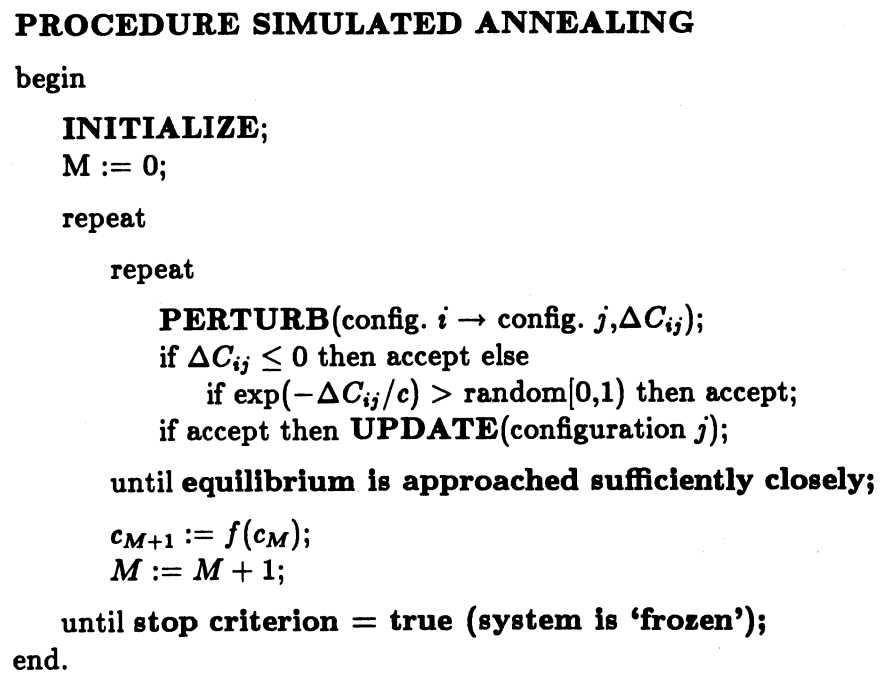
\includegraphics[width=1\textwidth]{./dados/figuras/procedure_simulated_annealing}
	\fonte{Figura 2.1 de \citeonline{van_1987}}
	\label{fig:procedure}
\end{figure}

No algoritmo \ref{alg:otimizadorInicial}, o valor da taxa de resfriamento é de 0,99, sendo a temperatura inicial e o número de passos por iteração escolhidos empiricamente. Sobre a temperatura inicial, esta deve receber um valor suficientemente alto para que possibilite as diversas trocas de posições da grade horária para a geração de uma solução satisfatória, mas não tão alto a ponto de fazer o algoritmo passar boa parte do tempo de execução realizando trocas aleatórias. Este valor 
pode ser definido empiricamente, ou utilizando o método explicitado por \citeonline{abramsomCooling}, em que é calculada a temperatura em que as soluções passam por uma transição de fase.

Explicando melhor o algoritmo, o método ``CriaGradeInicial''  gera uma matriz com as turmas e números de aulas de cada professor alocados corretamente. Esta grade inicial provavelmente possui inúmeros conflitos, portanto são aplicados os passos de otimização. Para cada passo de otimização, são escolhidas aleatoriamente uma turma e duas linhas (posições) da grade horária. Com estas informações, é calculada a variação do número de conflitos que a permutação dos professores nas linhas escolhidas ocasionaria. 

De acordo com o valor de variação calculado (delta), é determinado se a troca dos professores deve ou não ser realizada: uma troca que diminua o número de conflitos sempre é aceita, enquanto uma troca que aumenta o número de conflitos pode ser aceita probabilistacamente, de acordo com o valor da temperatura na iteração atual.

Em relação à condição de parada, durante o desenvolvimento deste primeiro incremento optou-se por utilizar o esgotamento da temperatura, ou seja, o algoritmo finaliza sua execução assim que a temperatura atinge um valor próximo de zero, quando não ocorrem mais permutações de professores.


